\documentclass{article}
\usepackage[utf8]{inputenc}
\usepackage[italian]{babel}
\usepackage{graphicx}
\usepackage{xcolor}
\usepackage[a4paper,top=15mm, bottom=15mm, left=15mm, right=15mm]{geometry}

\begin{document}
	
	\title{Esercizi svolti diagramma ER}
	\author{Alessandro Fuser}
	\maketitle
	
	\pagebreak
	
	\tableofcontents
	
	\pagebreak
	
	\section{Problemi}
	\subsection{Università}
	Un'università vuole raccogliere ed organizzare le informazioni sui propri studenti in relazione ai corsi che essi frequentano ed agli esami che essi sostengono. Uno studente è rappresentato da un nome, un cognome ed una matricola. Ogni corso viene etichettato con un nome, un professore che la insegna e un numero di CFU.
	\begin{enumerate}
		\item Disegnare il modello E/R
		\item Verificare lo schema con le regole di lettura
		\item Costruisci il corrispondente schema logico
	\end{enumerate}
	Rispondi alle seguenti domande in SQL:
	\begin{itemize}
		\item Crea le tabelle dello schema logico
		\item Inserisci un'istanza in una tabella
		\item Visualizza tutti gli studenti che si chiamano "Marco"
		\item Visualizza tutti i corsi tenuti dal professor "Roncaccioli"
		\item Visualizza quanti esami da 6 CFU sono stati effettuati
	\end{itemize}
	
	\subsection{Analisi dei consumi}
	Una società di analisi dei consumi vuole controllare gli acquisti fatti dai clienti presso una loro negozio. Ogni utente possiede una tessera personale dove tiene i punti fedeltà. I prodotti acquistati hanno un codice a barre, un nome ed una descrizione. I negozi sono dislocati con indirizzi diversi, che li identificano. Ogni acquisto viene registrato sulla tessera e vengono aggiunti i corrispettivi punti. Ogni negozio ha un proprio listino e può proporre prezzi diversi per gli stessi prodotti.
	\begin{enumerate}
		\item Disegnare il modello E/R
		\item Verificare lo schema con le regole di lettura
		\item Costruisci il corrispondente schema logico
	\end{enumerate}
	Rispondi alle seguenti domande in SQL:
	\begin{itemize}
		\item Crea le tabelle dello schema logico
		\item Inserisci un'istanza in una tabella
		\item Visualizza i punti delle tessere degli utenti
		\item Visualizza tutti i prodotti di un negozio in "Viale Trento 12"
		\item Visualizza tutti i prodotti acquistati dall'utente "U154"
	\end{itemize}
	
	\subsection{Pratiche degli impiegati}
	Si vuole organizzare un sondaggio in merito al lavoro degli impiegati nello svolgimento delle pratiche. Queste vengono individuate tramite un codice ed un argomento da scegliere tra "automobilistica", "previdenziale" e "sanitaria". Il sondaggio vuole tenere conto anche delle città italiane in cui lavorano gli impiegati, contraddistinte da un nome e da un CAP. Degli impiegati vogliamo sapere il nome, il cognome ed il ruolo aziendale.
	\begin{enumerate}
		\item Disegnare il modello E/R
		\item Verificare lo schema con le regole di lettura
		\item Costruisci il corrispondente schema logico
	\end{enumerate}
	Rispondi alle seguenti domande in SQL:
	\begin{itemize}
		\item Crea le tabelle dello schema logico
		\item Inserisci un'istanza in una tabella
		\item Visualizza tutte le pratiche di tipo "previdenziale"
		\item Visualizza tutti gli impiegati che lavorano a Milano
		\item Visualizza tutte le pratiche svolte dai dirigenti
	\end{itemize}

	\subsection{Società polisportiva}
	Una società polisportiva vuole organizzare dei corsi tenuti da propri istruttori. Di questi si vuole conoscere il nome, il cognome e le ore svolte nella palestra. Ogni corso è contraddistinto da un nome, da un istruttore che lo tiene e da un orario. Ogni corso è specifico per una disciplina ed è frequentato da soci della società. Di un socio si tiene traccia del nominativo, del numero corsi che tiene ed è identificato dal proprio numero di tessera.
	\begin{enumerate}
		\item Disegnare il modello E/R
		\item Verificare lo schema con le regole di lettura
		\item Costruisci il corrispondente schema logico
	\end{enumerate}
	Rispondi alle seguenti domande in SQL:
	\begin{itemize}
		\item Crea le tabelle dello schema logico
		\item Inserisci un'istanza in una tabella
		\item Visualizza le ore svolte dagli istruttori
		\item Visualizza i corsi svolti da un istruttore chiamato "Gesù"
		\item Visualizza le disciplina a cui appartiene un socio chiamato "Paolo"
	\end{itemize}

	\subsection{Negozi}
	Una catena di negozi è costituita da un certo numero di centri vendita di cui interessano il codice, la ragione sociale e l’indirizzo. I centri vendita effettuano ordini (caratterizzati da un codice e dalla data d’ordine) che comprendono gli articoli da vendere, i quali appartengono a diverse categorie merceologiche (ad esempio“alimentari”, “abbigliamento” ecc.).
	\begin{enumerate}
		\item Disegnare il modello E/R
		\item Verificare lo schema con le regole di lettura
		\item Costruisci il corrispondente schema logico
	\end{enumerate}
	Rispondi alle seguenti domande in SQL:
	\begin{itemize}
		\item Crea le tabelle dello schema logico
		\item Inserisci un'istanza in una tabella
		\item Visualizza tutti gli articoli alimentari
		\item Visualizza tutti i centri vendita che hanno fatto un ordine il 01/01/2018
		\item Visualizza tutti i prodotti dell'ordine "O002"
	\end{itemize}

	\subsection{Noleggio DVD}
	Una società che gestisce un noleggio di film dvd vuole organizzare un database a fini statistici. Ogni noleggio è individuato dal codice e dalla data di noleggio. A tale scopo è interessata a catalogare i suoi clienti tramite il numero di tessera, il nominativo e la data di nascita. Inoltre di ogni dvd sono noti il titolo ed il regista, oltre le informazioni utili allo scopo.
	\begin{enumerate}
		\item Disegnare il modello E/R
		\item Verificare lo schema con le regole di lettura
		\item Costruisci il corrispondente schema logico
	\end{enumerate}
	Rispondi alle seguenti domande in SQL:
	\begin{itemize}
		\item Crea le tabelle dello schema logico
		\item Inserisci un'istanza in una tabella
		\item Visualizza tutti i clienti nati prima del 1970
		\item Visualizza tutti registi "noleggiati" da un cliente
		\item Visualizza tutti i dvd presenti in un noleggio
	\end{itemize}

	\subsection{Opere d'arte}
	Si vuole organizzare un database che archivi le opere d’arte presenti nei musei italiani. Tali opere sono identificate tramite un codice identificativo, il titolo ed il valore commerciale. Il database vuole gestire anche un’anagrafica degli artisti che sono esposti nei musei italiani ed un’anagrafica delle città italiane viste sia come sede dei musei stessi, sia come luogo di nascita degli artisti.
	\begin{enumerate}
		\item Disegnare il modello E/R
		\item Verificare lo schema con le regole di lettura
		\item Costruisci il corrispondente schema logico
	\end{enumerate}
	Rispondi alle seguenti domande in SQL:
	\begin{itemize}
		\item Crea le tabelle dello schema logico
		\item Inserisci un'istanza in una tabella
		\item Visualizza tutti gli artisti esposti
		\item Visualizza tutte le opere esposte di artisti nati a "Padova"
		\item Visualizza il valore commerciale di ogni opera della città di "Vicenza"
	\end{itemize}

	\subsection{Ospedale}
	Un ospedale è composto da reparti. A un reparto afferiscono (ossia sono presenti) medici. Un paziente può essere ricoverato in un reparto e si tiene traccia del suo codice, nome, cognome, codice fiscale, data e luogo di nascita, sesso, data di ricovero. Di un medico si memorizza codice, nome, cognome, data e luogo di nascita. I medici effettuano visite sui pazienti. I pazienti subiscono le visite. Di una visita si memorizza la data e l’esito. Sui pazienti, inoltre, vengono effettuati esami di laboratorio. Di un esame si memorizza il tipo, la data e l’esito. NB: un medico può visitare un paziente più volte in date diverse, quindi modella le visite come entità
	\begin{enumerate}
		\item Disegnare il modello E/R
		\item Verificare lo schema con le regole di lettura
		\item Costruisci il corrispondente schema logico
	\end{enumerate}
	Rispondi alle seguenti domande in SQL:
	\begin{itemize}
		\item Crea le tabelle dello schema logico
		\item Inserisci un'istanza in una tabella
		\item Visualizza tutte le visite svolte da un paziente
		\item Visualizza il nome di tutti i pazienti ricoverati nel reparto di pediatria
	\end{itemize}
	\pagebreak
	
	\section{Soluzioni}
	\subsection{Università}
	\subsubsection{Modello ER}
	\begin{figure}[h!]
		\centering
		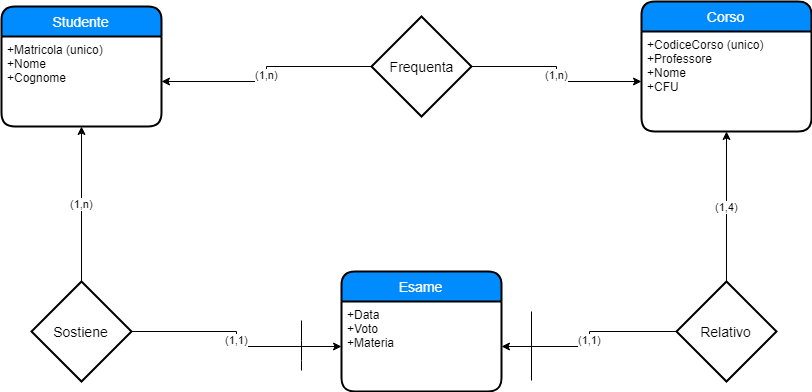
\includegraphics[scale=0.5]{images/Universita.png}
	\end{figure}
	\subsubsection{Regole di lettura}
	\begin{itemize}
		\item Ogni studente sostiene uno o più esami ed ogni esame deve essere sostenuto da un solo studente
		\item Ogni studente può frequentare più corsi ed un corso può essere frequentato da più studenti
		\item Ogni esame è relativo ad un solo corso ed per un corso ci possono essere al massimo 4 esami
	\end{itemize}
	\subsubsection{Schema Logico}
	Studente(\underline{Matricola}, Nome, Cognome)\\
	Corso(\underline{CodiceCorso}, Professore, Nome, CFU)\\
	Esame(Data, Voto, Materia, \underline{Matricola}, \underline{CodiceCorso})\\
	Frequenta(\underline{Matricola}, \underline{CodiceCorso})
	\subsubsection{SQL}
	\begin{verbatim}
		SELECT Matricola
		FROM Studente
		WHERE Studente.Nome = "Marco"
	\end{verbatim}
	\begin{verbatim}
		SELECT CodiceCorso
		FROM Corso
		WHERE Corso.Professore = "Roncaccioli"
	\end{verbatim}
	\begin{verbatim}
		SELECT CodiceCorso, Matricola, Data, Materia
		FROM Esame, Corso
		WHERE Esame.CodiceCorso = Corso.CodiceCorso AND Corso.CFU = 6
	\end{verbatim}

	\pagebreak
	
	\subsection{Analisi dei consumi}
	\subsubsection{Modello ER}
	\begin{figure}[h!]
		\centering
		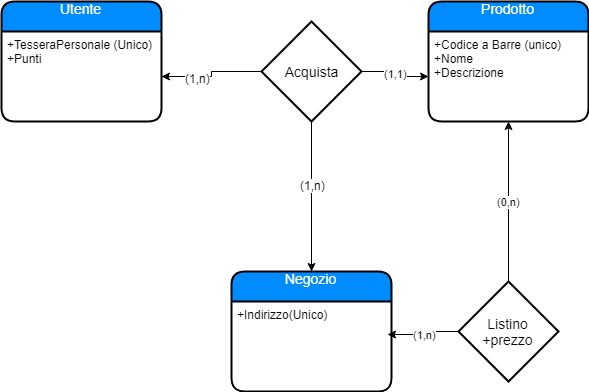
\includegraphics[scale=0.5]{images/AnalisiConsumi.png}
	\end{figure}
	\subsubsection{Regole di lettura}
	\begin{itemize}
		\item Un cliente può acquistare più prodotti nello stesso negozio, in negozio ci sono più clienti che acquistano dei prodotti ed un prodotto può essere acquistato da più clienti in diversi negozi
		\item Un negozio ha nel proprio listino diversi prodotti ed un prodotto può essere in dei listini
	\end{itemize}
	\subsubsection{Schema Logico}
	Utente(\underline{TesseraPersonale}, Punti)\\
	Prodotto(\underline{CodiceABarre}, Nome, Descrizione, \underline{TesseraPersonale}, \underline{Indirizzo})\\
	Negozio(\underline{Indirizzo})\\
	Listino+Prezzo(\underline{CodiceABarre}, \underline{Indirizzo})\\
	\subsubsection{SQL}
	\begin{verbatim}
	SELECT Punti
	FROM Utente
	\end{verbatim}
	\begin{verbatim}
	SELECT CodiceABarre, Nome
	FROM Listino+Prezzo, Prodotto
	WHERE Listino+Prezzo.CodiceABarre = Prodotto.CodiceABarre AND Listino+Prezzo.CodiceABarre = "Viale Trento 12"
	\end{verbatim}
	\begin{verbatim}
	SELECT CodiceABarre, Nome
	FROM Prodotto, Utente
	WHERE Prodotto.TesseraPersonale = Utente.TesseraPersonale AND Prodotto.TesseraPersonale = "U154"
	\end{verbatim}
	
	\pagebreak
	\subsection{Pratiche degli impiegati}
	\subsubsection{Modello ER}
	\begin{figure}[h!]
		\centering
		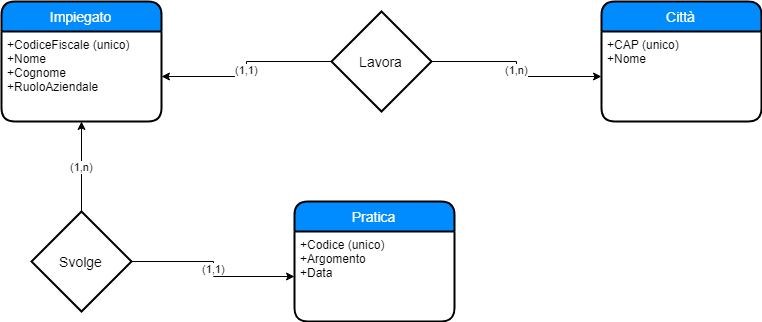
\includegraphics[scale=0.5]{images/ImpiegatiPratica.png}
	\end{figure}
	\subsubsection{Regole di lettura}
	\begin{itemize}
		\item Un impiegato può lavorare in una sola città e in una città possono lavorare più impiegati
		\item Un impiegato può svolgere più pratiche e una pratica può essere svolta da un solo impiegato
	\end{itemize}
	\subsubsection{Schema Logico}
	Impiegato(\underline{CodiceFiscale}, Nome, Cognome, RuoloAziendale, \underline{CAP})\\
	Città(\underline{CAP}, Nome)\\
	Pratica(\underline{Codice}, Argomento, Data, \underline{CodiceFiscale})
	\subsubsection{SQL}
	\begin{verbatim}
	SELECT Codice, Argomento
	FROM Pratica
	WHERE Pratica.Argomento = "Previdenziale"
	\end{verbatim}
	\begin{verbatim}
	SELECT CodiceFiscale, Nome, CAP
	FROM Impiegato, Città
	WHERE Impiegato.CAP = Città.CAP AND Città.Nome = "Milano"
	\end{verbatim}
	\begin{verbatim}
	SELECT Codice, RuoloAziendale
	FROM IMpiegato, Pratica
	WHERE Pratica.CodiceFiscale = Impiegato.CodiceFiscale AND Impiegato.RuoloAziendale = "Dirigente"
	\end{verbatim}

	\pagebreak
	
	\subsection{Società polisportiva}
	\subsubsection{Modello ER}
	\begin{figure}[h!]
		\centering
		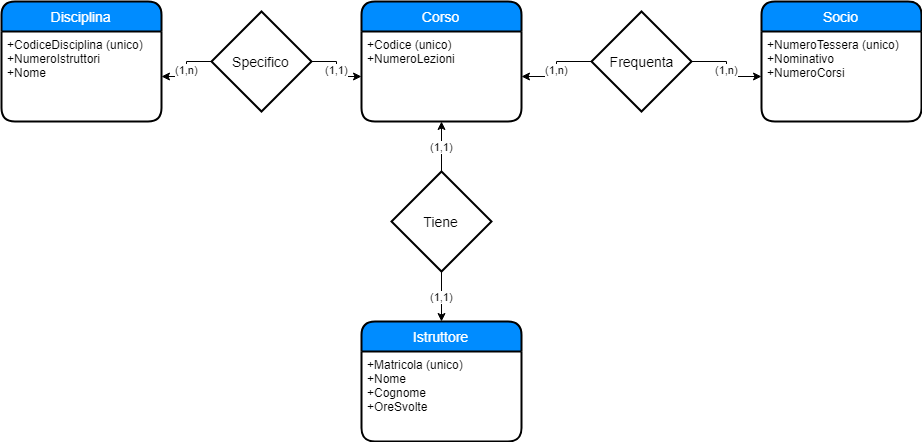
\includegraphics[scale=0.5]{images/Palestra.png}
	\end{figure}
	\subsubsection{Regole di lettura}
	\begin{itemize}
		\item Una disciplina può avere al suo interno più corsi ma un corso può appartenere ad una sola disciplina
		\item Un corso può essere frequentato da più soci ed un socio può frequentare più corsi
		\item Un corso è tenuto da un solo istruttore ed un istruttore può tenere un solo corso
	\end{itemize}
	\subsubsection{Schema Logico}
	Disciplina(\underline{CodiceDisciplina}, NumeroIstruttori, Nome)\\
	Corso(\underline{Codice}, NumeroLezioni, \underline{Matricola}, Nome, Cognome, OreSvolte, \underline{CodiceDisciplina})\\
	Socio(\underline{NumeroTessera}, Nominativo, NumeroCorsi)\\
	Frequenta(\underline{Codice}, \underline{NumeroTessera})
	\subsubsection{SQL}
	\begin{verbatim}
	SELECT Matricola, OreSvolte
	FROM Corso
	\end{verbatim}
	\begin{verbatim}
	SELECT Codice, Matricola, Nome
	FROM Corso
	WHERE Corso.Nome = "Gesù"
	\end{verbatim}
	\begin{verbatim}
	SELECT CodiceDisciplina, NomeDisciplina, NumeroTessera, Nominativo
	FROM Disciplina, Corso, Frequenta, Socio
	WHERE Disciplina.CodiceDisciplina = Corso.CodiceDisciplina AND Corso.Codice = Frequente.Codice
		AND Frequenta.NumeroTessera = Socio.NumeroTessera AND Socio.Nominativo = "Paolo"
	\end{verbatim}

	\pagebreak
	
	\subsection{Negozi}
	\subsubsection{Modello ER}
	\begin{figure}[h!]
		\centering
		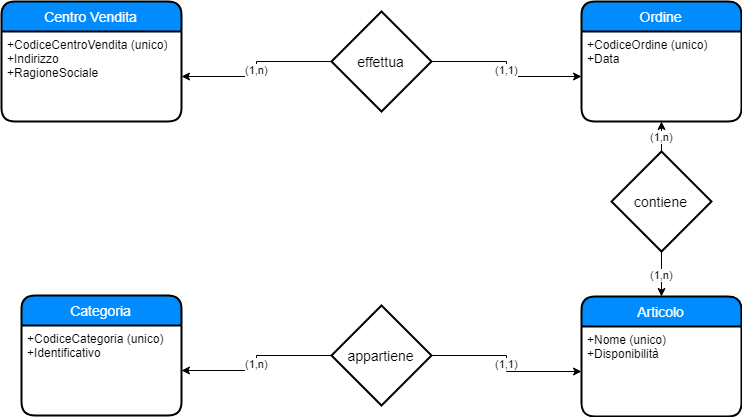
\includegraphics[scale=0.5]{images/Negozio.png}
	\end{figure}
	\subsubsection{Regole di lettura}
	\begin{itemize}
		\item Un Centro Vendita può effettuare più ordini ma un ordine può essere fatto da un solo centro vendita
		\item Un ordine può contenere più articolo ed un articolo può essere in più ordini
		\item Un articolo può appartenere solo ad una categoria ma una categoria può avere più articoli al suo interno
	\end{itemize}
	\subsubsection{Schema Logico}
	CentroVendita(\underline{CodiceCentroVendita}, Indirizzo, RagioneSociale)\\
	Ordine(\underline{CodiceOrdine}, Data, \underline{CodiceCentroVendita})\\
	Articolo(\underline{Nome}, Disponibilità, \underline{CodiceCategoria})\\
	Categoria(\underline{CodiceCategoria}, Identificativo)\\
	Contiene(\underline{CodiceOrdine}, \underline{Nome})
	\subsubsection{SQL}
	\begin{verbatim}
	SELECT Nome, , CodiceCategoria, Identificativo
	FROM Articolo, Categoria
	WHERE Articolo.CodiceCategoria = Categoria.CodiceCategoria AND Categoria.Identificativo = "Alimentare"
	\end{verbatim}
	\begin{verbatim}
	SELECT CodiceCentroVendita, Data, Indirizzo
	FROM Ordine, CentroVendita
	WHERE Ordine.Data = "01/01/2018" AND Ordine.CodiceCentroVendita = CentroVendita.CodiceCentroVendita
	\end{verbatim}
	\begin{verbatim}
	SELECT CodiceOrdine, Nome
	FROM Contiene
	WHERE Contiene.CodiceOrdine = "O002"
	\end{verbatim}

	\pagebreak
	
	\subsection{Noleggio DVD}
	\subsubsection{Modello ER}
	\begin{figure}[h!]
		\centering
		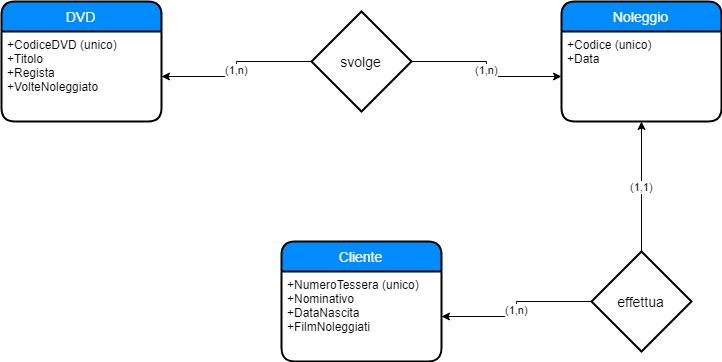
\includegraphics[scale=0.5]{images/NoleggioDVD.png}
	\end{figure}
	\subsubsection{Regole di lettura}
	\begin{itemize}
		\item Un DVD può essere noleggiato più volte ed in un noleggio si possono prendere più DVD
		\item Un noleggio può essere fatto da un solo cliente ma un cliente può effettuare più noleggi
	\end{itemize}
	\subsubsection{Schema Logico}
	DVD(\underline{CodiceDVD}, Titolo, Regista, VolteNoleggiato)\\
	Noleggio(\underline{Codice}, Data, \underline{NumeroTessera})\\
	Cliente(\underline{NumeroTessera}, Nominativo, DataNascita, FilmNoleggiati)\\
	Svolge(\underline{CodiceDVD}, \underline{Codice})
	\subsubsection{SQL}
	\begin{verbatim}
	SELECT NumeroTessera, Nominativo, DataNascita
	FROM Cliente
	WHERE Cliente.DataNascita < "01/01/1970"
	\end{verbatim}
	\begin{verbatim}
	SELECT NumeroTessera, Nominativo, Codice, CodiceDVD, Regista
	FROM Cliente, Noleggio, Svolge, DVD
	WHERE Cliente.NumeroTessera = Noleggio.NumeroTessera AND Noleggio.Codice = Svolge.Codice 
	AND Svolge.CodiceDVD = DVD.CodiceDVD 
	\end{verbatim}
	\begin{verbatim}
	SELECT CodiceDVD, Codice, Titolo
	FROM DVD, Svolge, Noleggio
	WHERE DVD.CodiceDVD = Svolge.Codice AND Noleggio.Codice = Svolge.Codice
	\end{verbatim}

	\pagebreak
	
	\subsection{Opere d'arte}
	\subsubsection{Modello ER}
	\begin{figure}[h!]
		\centering
		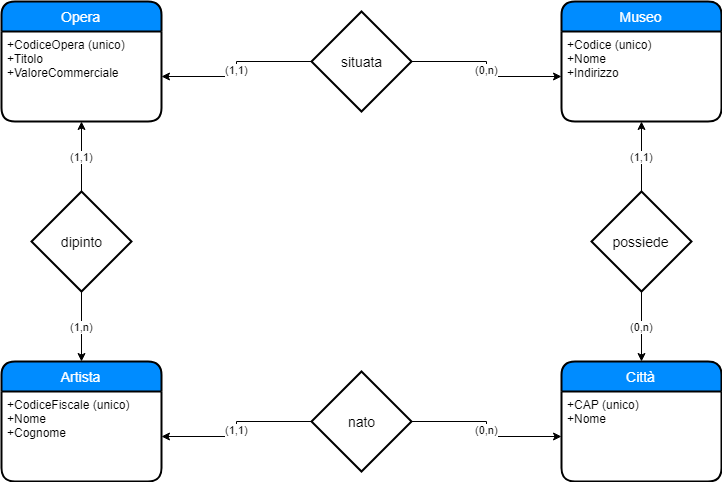
\includegraphics[scale=0.5]{images/Opera.png}
	\end{figure}
	\subsubsection{Regole di lettura}
	\begin{itemize}
		\item Un'opera deve essere esposta in un solo museo ed un museo può avere più opere esposte
		\item Un museo è situato in una sola città e una città può avere dei musei
		\item Un artista deve essere nato in una città e una città può aver dato i natali a degli artisti
		\item Un artista ha dipinto una o più opere ed un'opera deve essere stata dipinta da un solo artista
	\end{itemize}
	\subsubsection{Schema Logico}
	Opera(\underline{CodiceOpera}, Titolo, ValoreCommerciale, \underline{Codice}, \underline{CodiceFiscale})\\
	Museo(\underline{Codice}, Nome, Indirizzo, \underline{CAP})\\
	Città(\underline{CAP}, Nome)\\
	Artista(\underline{CodiceFiscale}, Nome, Cognome, \underline{CAP})
	\subsubsection{SQL}
	\begin{verbatim}
	SELECT CodiceFiscale, Nome, Cognome
	FROM Artista
	\end{verbatim}
	\begin{verbatim}
	SELECT CodiceOpera, Titolo, CodiceFiscale, Cap, NomeCittà
	FROM Opera, Artista, Città
	WHERE Opera.CodiceFiscale = Artista.CodiceFiscale AND Artista.CAP = Città.CAP AND Città.Nome = "Padova"
	\end{verbatim}
	\begin{verbatim}
	SELECT CodiceOpera, ValoreCommerciale, Codice, CAP, Nome
	FROM Opera, Museo, Città
	WHERE Opera.Codice = Mueso.Codice AND Museo.CAP = Città.CAP AND Città.Nome = "Vicenza"
	\end{verbatim}

	\pagebreak
	
	\subsection{Ospedale}
	\subsubsection{Modello ER}
	\begin{figure}[h!]
		\centering
		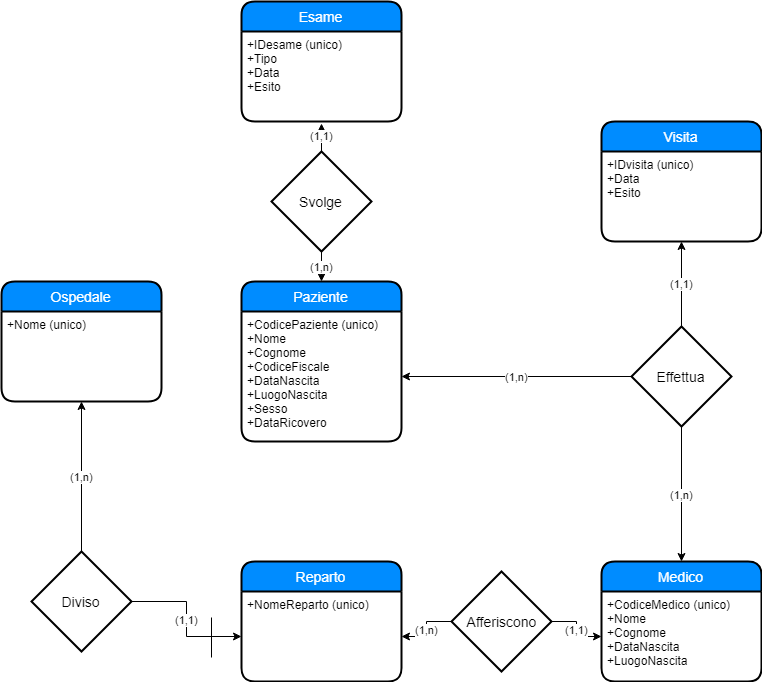
\includegraphics[scale=0.5]{images/Ospedale.png}
	\end{figure}
	\subsubsection{Regole di lettura}
	\begin{itemize}
		\item In un ospedale ci sono più reparti ma un reparto può appartenere ad un solo ospedale particolare (da qui entità debole)
		\item In un reparto afferiscono più medici, un medico appartiene ad un solo reparto
		\item Un paziente può fare più esami, un esame può essere fatto solo su un paziente
		\item Un paziente può effettuare più visite con un dottore, una visita può essere condotta da un solo medico su un solo paziente, un medico può fare fare più visite su più pazienti
	\end{itemize}
	\subsubsection{Schema Logico}
	Ospedale(\underline{Nome})\\
	Reparto(\underline{NomeReparto}, \underline{Nome})\\
	Medico(\underline{CodiceMedico}, Nome, Cognome, DataNascita, LuogoNascita, \underline{NomeReparto})\\
	Visita(\underline{IDvisita}, Data, Esito, \underline{CodiceMedico}, \underline{CodicePaziente})\\
	Paziente(\underline{CodicePaziente}, Nome, Cognome, CodiceFiscale, DataNascita, LuogoNascita, Sesso, DataRicovero)\\
	Esame(\underline{IDesame}, Tipo, Data, Esito, \underline{CodicePaziente})
	\subsubsection{SQL}
	\begin{verbatim}
	SELECT CodicePaziente, IDVisita
	FROM Visita
	\end{verbatim}
	\begin{verbatim}
	SELECT CodicePaziente, Nome, IDVisita, CodiceMedico, NomeReparto
	FROM Paziente, Visita, Medico
	WHERE Paziente.CodicePaziente = Visita.CodicePaziente AND Visita.CodiceMedico = Meedico.CodiceMedico
	AND Medico.NomeReparto = "Pediatria"
	\end{verbatim}

\end{document}